% !TEX root = ../main.tex

%%% ============================================================
\section{Thực nghiệm: thu thập, phân tích và diễn giải dữ liệu}
%%% ============================================================

\subsection{Pipeline thu thập dữ liệu}
\begin{frame}{Pipeline HSGE: vòng lặp khám phá $\rightarrow$ thu thập dữ liệu}
  \begin{center}
    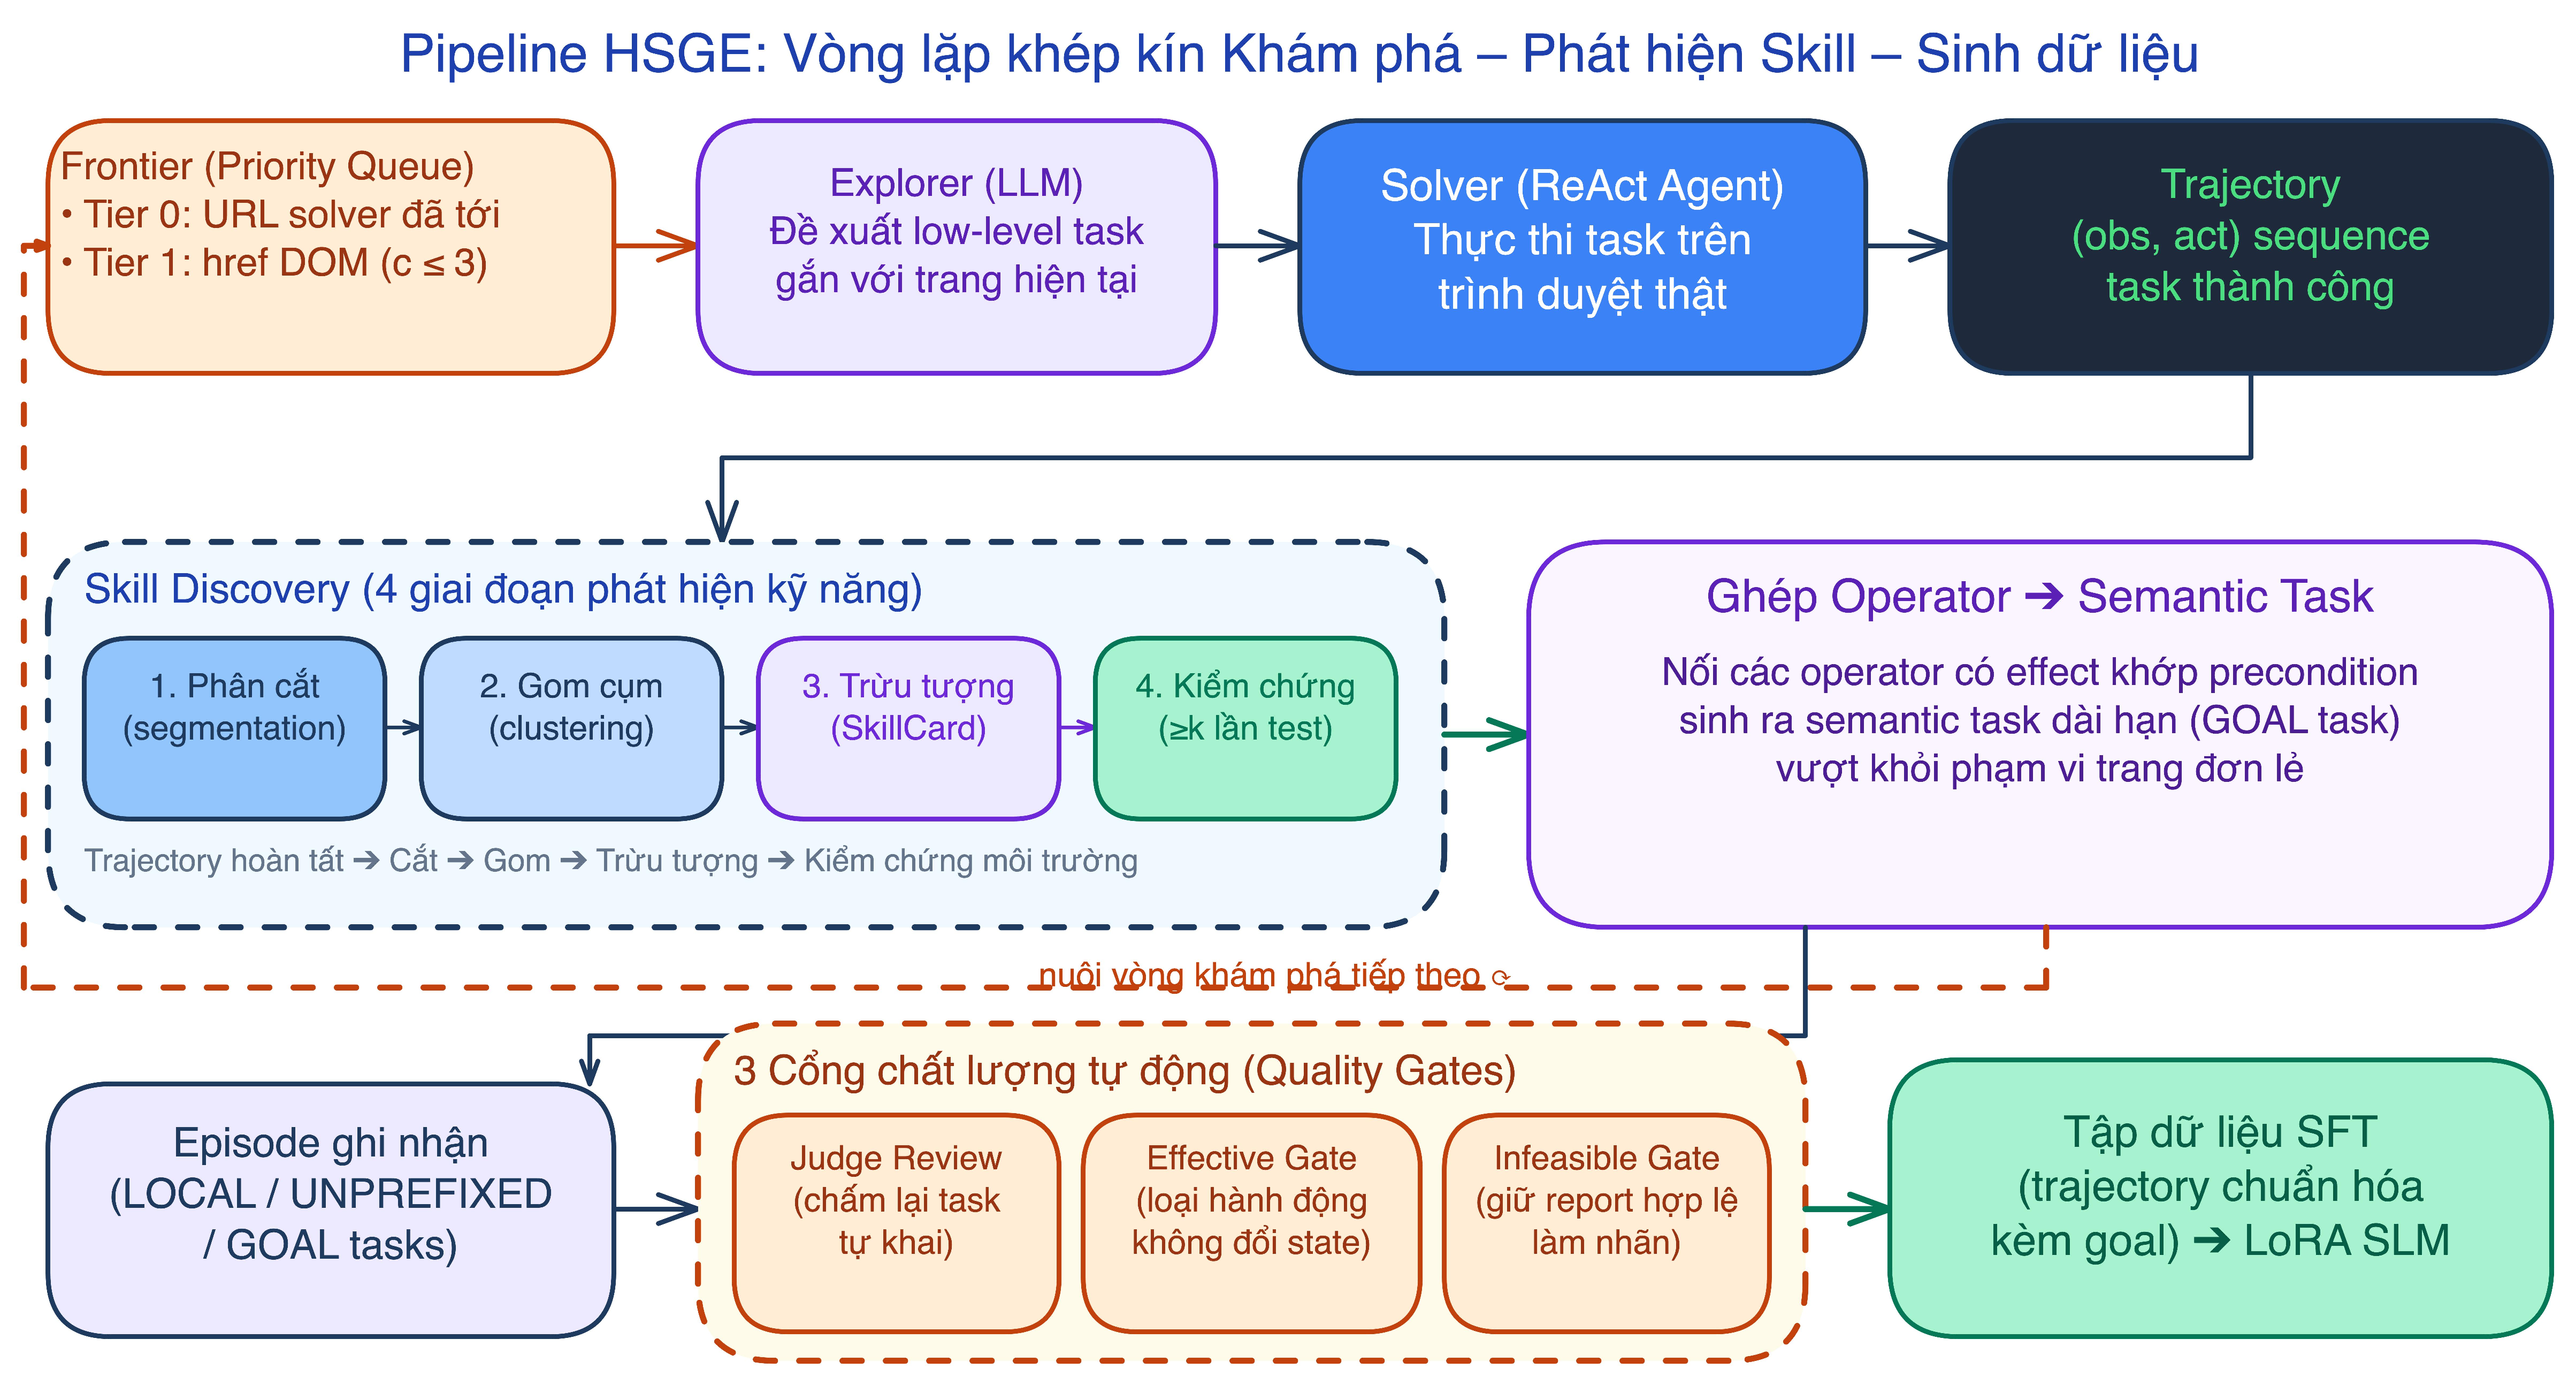
\includegraphics[width=\linewidth,height=0.62\textheight,keepaspectratio]{fig_pipeline.pdf}
  \end{center}
  \figcap{Vòng lặp khép kín: Khám phá $\rightarrow$ Phát hiện skill $\rightarrow$ Quy nạp operator $\rightarrow$ Ghép semantic task $\rightarrow$ Tinh lọc dữ liệu.}
\end{frame}

\subsection{Thiết lập \& phễu dữ liệu}
\begin{frame}{Thiết lập thực nghiệm và phễu dữ liệu thu được}
  \begin{columns}[t]
    \begin{column}{0.46\textwidth}
      \footnotesize
      \textbf{Thiết lập}
      \begin{itemize}\setlength{\itemsep}{3pt}
        \item \textbf{Môi trường}: 4 website WebArena tự triển khai (Shopping, Shopping Admin, GitLab, Reddit).
        \item \textbf{Khám phá}: 4 đợt ($\approx$21h/site), \kw{20\,808 lượt gọi LLM}.
        \item \textbf{Đánh giá}: \kw{655 task chính thức}, chấm tự động, 15 bước/task, \texttt{temperature}$=0$.
        \item \textbf{Huấn luyện}: Qwen3.5-9B $+$ LoRA, 1119 bước (5h09).
      \end{itemize}
    \end{column}
    \begin{column}{0.52\textwidth}
      \footnotesize
      \textbf{Phễu dữ liệu} (4 website)
      \vspace{0.03cm}

      \scriptsize
      \begin{tabular}{@{}L{4.2cm} R{1.4cm}@{}}
        \toprule
        Node đã duyệt (71 trùng lặp) & \textbf{455} \\
        Episode ghi nhận & \textbf{3981} \\
        Episode hợp lệ sau kiểm chứng & \textbf{2117} (53,2\%) \\
        \midrule
        Skill thu nhận / Operator quy nạp & \textbf{146 / 57} \\
        Semantic task sinh ra & \textbf{142} \\
        \midrule
        Trajectory vào dataset & \textbf{1760} \\
        Mẫu huấn luyện (Train/Val) & \textbf{8554 / 453} \\
        \bottomrule
      \end{tabular}
      {\scriptsize \kw{0} mục tiêu trùng train/val, \kw{0} nhãn từ con người. Chi phí API: \textbf{\$36,48}.}
    \end{column}
  \end{columns}
\end{frame}

\subsection{Phân tích \& diễn giải kết quả}
\begin{frame}{Kết quả chính trên 655 task và diễn giải}
  \centering
  \footnotesize
  \setlength{\tabcolsep}{4pt}
  \begin{table}
    \begin{tabular}{@{}L{2.6cm} R{2.5cm} R{2.5cm} R{1.6cm} R{2.0cm}@{}}
      \toprule
      \textbf{Website} & \textbf{Mô hình nền} & \textbf{Sau fine-tune} &
      \textbf{Chênh lệch} & \textbf{$p$ (McNemar)} \\
      \midrule
      Shopping       & 37/187 $=$ 19,8\% & 53/187 $=$ 28,3\% & $+$8,6  & 0,011 \\
      Reddit         & 7/106 $=$ 6,6\%   & 36/106 $=$ 34,0\% & $+$27,4 & $<$0,001 \\
      GitLab         & 20/180 $=$ 11,1\% & 33/180 $=$ 18,3\% & $+$7,2  & 0,011 \\
      Shopping Admin & 23/182 $=$ 12,6\% & 39/182 $=$ 21,4\% & $+$8,8  & 0,005 \\
      \midrule
      \textbf{Tổng} & \textbf{87/655 $=$ 13,3\%} & \textbf{161/655 $=$ 24,6\%} &
      \kw{$+$11,3\%} & \kw{$<$0,001} \\
      \bottomrule
    \end{tabular}
  \end{table}

  \vspace{0.1cm}
  \begin{columns}[t]
    \begin{column}{0.48\textwidth}
      \scriptsize
      \textbf{Đánh giá công bằng, nghiêm ngặt}: cùng tập task, prompt, ngân sách bước, bộ chấm. McNemar theo cặp: \kw{100 task} chỉ mô hình fine-tune giải được (vs 26 task mô hình nền).
    \end{column}
    \begin{column}{0.48\textwidth}
      \scriptsize
      \textbf{Diễn giải}: ý nghĩa thống kê trên \kw{toàn bộ 4/4 website} ($p \le 0{,}011$); lỗi định dạng đầu ra giảm từ 26,0\% xuống 0,6\% $\Rightarrow$ SLM làm chủ giao diện hành động.
    \end{column}
  \end{columns}
\end{frame}

\subsection{Minh họa thực thi (Demo)}
\begin{frame}{Demo: mô hình sau fine-tune giải một task WebArena}
  \begin{columns}[c]
    \begin{column}{0.42\textwidth}
      \footnotesize
      \textbf{Đặc điểm thực thi}
      \begin{itemize}\setlength{\itemsep}{4pt}
        \item \textbf{Đầu vào}: chỉ URL $+$ accessibility tree (không dùng ảnh).
        \item \textbf{Định dạng chuẩn}: sinh \texttt{thought} và \texttt{action} chuẩn xác.
        \item \textbf{Tự động chấm}: benchmark chính thức tự kiểm chứng hoàn thành task.
      \end{itemize}
    \end{column}
    \begin{column}{0.56\textwidth}
      \centering
      \setbeamercolor{demoframe}{bg=structure.fg!8,fg=structure.fg}
      \begin{beamercolorbox}[wd=\linewidth,ht=0.5\textheight,center]{demoframe}
        \vfill
        {\large \textbf{[\,DEMO TRỰC TIẾP / VIDEO\,]}}\\[0.3cm]
        {\footnotesize Chạy trực tiếp một vòng khám phá + giải task, hoặc video quay sẵn}
        \vfill
      \end{beamercolorbox}
    \end{column}
  \end{columns}
\end{frame}
